\section{Lithium-Ion Batteries}
\label{Chap:lithium_ion_batteries}
Before a battery is chosen and investigated in detail, it is important to know exactly how such a battery works. Key parameters have to be explained and the many different options of batteries have to be discussed. In this section, a general explanation of lithium-ion batteries will be given as well as an explanation of some common commercial configurations in which they come.

\subsection{What is a lithium-ion battery}
Lithium-ion batteries work like most other batteries available. Batteries now-a-days consist out of a cathode, anode, electrolyte, separator and current collectors. A schematic drawing of a battery layer is given in figure \ref{Fig:Li-Ion_Schematic}.

\begin{figure} [H]
 	\centering	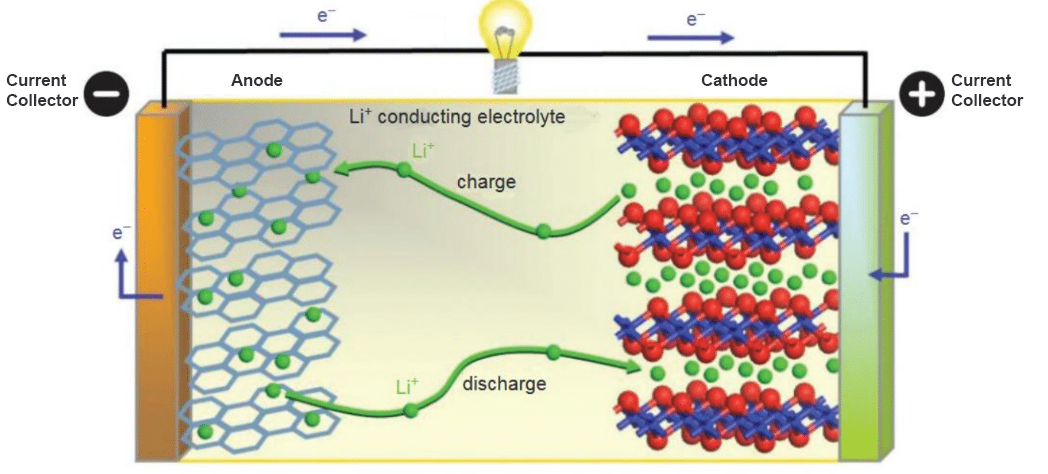
\includegraphics[width=0.8\linewidth]{Figures/scematic.PNG}
 	\caption{Schematic drawing of the lithium-ion battery layer}
    \label{Fig:Li-Ion_Schematic}
\end{figure}

When discharging, lithium-ion particles (hence lithium-ion batteries) flow from the anode to the cathode material. The anode and cathode material is structured so that the lithium-ion particles can be released and taken into the layered structure. A process called intercalation. Some common materials that inherit this structure are carbon compounds like graphite for the anode, and metallic oxides like LiCoO$_2$ for the cathode. When the charged lithium particles transfer from anode to cathode, an potential difference is created causing electrons to flow as well.

However, electrons need to flow through an external circuit, as to allow some device to be powered. Thus a non-conductive barrier must be created that allows lithium-ions to be transferred, but stops electrons from going through. An aqueous medium called the electrolyte allows the transfer of lithium particles. This medium is a lithium salt like LiPF$_6$ which is solved into a EC:DEC:DMC solvent usually. The specific materials and ratios used may vary however. A porous polymer membrane gelled with this electrolyte is then placed in the middle of the electrodes. This allows lithium-ions to travel through, but stops electrons from doing so.

The electrodes are coated onto metal current collectors. Current collectors form the positive and negative terminal of a battery. Because of the potential difference in the electrodes, electrons then flow through the current collector through the external circuit and back into the battery again, equaling the potential difference (causing a voltage drop explained in \textbf{REFERENEN NAAR VOLTAGE DROP}).

Typically, a battery's electrodes are defined during discharge. When someone refers to the cathode material, this means the person refers to the material that is the cathode during discharge. However during charge, the electrodes switch. The discharging anode becomes the charging cathode, and the other way around for the discharging cathode. During charge, lithium ions flow back to their original side. This is the mechanism that allows lithium batteries to be recharged. A problem however is that lithium batteries have only a limited amount of recharges after which they become unstable and a lacking performance. This is due to mechanism described later in section \ref{Chap:Battery_Safety}.

\subsection{Chemistries}
There are many different lithium battery commercially available. They mostly differ in mechanical structure and in their chemistry. Both may have a significant impact on battery performance. First, a select few popular commercial chemistries will be looked into, after which different mechanical structures will be detailed. 

Although all components of a lithium battery can be changed in material, manufacturers and data-sheets will almost always refer to the cathode material as to define the battery its chemistry. Why that is, is that all other components do not have good commercially available alternatives. Almost all anodes are made out of graphite. Today incorporating silicone additives into the graphene is ongoing, yet still commercially unavailable. Graphene also is being looked into, however still mainly graphite is used. \\
Cathode material however consists out of metal oxides, of which there are many different options. Each of these have different impact on the performance of a battery. Since mainly the cathode material impacts the batteries performance electrochemically, the cathode material is thus referred to as to define the batteries chemistry \cite{cathode}. The cathode impacts energy density, power density, safety and lifespan. Also choice of cathode impacts the costs, depending on the cathode material, it can make up 25$\%$ of the total battery production costs. \cite{cathode}\cite{cobalt}

\begin{figure} [H]
 	\centering
 	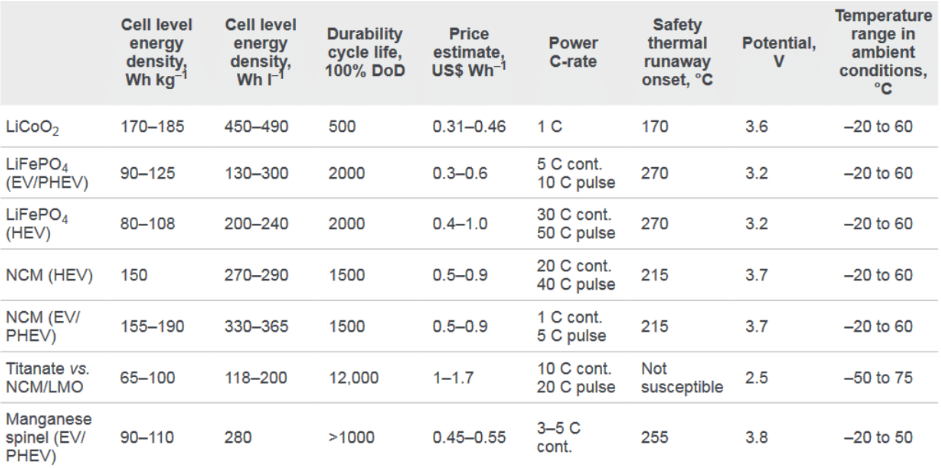
\includegraphics[width=0.9\linewidth]{Figures/chemistry_table.PNG}
 	\caption{Battery cell properties with different chemistries (from \cite{slides})}
    \label{Fig:Chemistry_table}
\end{figure}

In figure \ref{Fig:Chemistry_table}, a table is given that indicates different properties of battery cells with different cathode chemistries. Below, a few common chemistries will be explained.\\
\begin{enumerate}
\item LCO - LiCoO$_2$\\
The Lithium Cobalt Oxide (LCO) chemistry is the most common type of lithium-ion battery. It owes its popularity by the high energy density both by weight and volume. In fact, by volume it inherits one of the highest energy densities. This is really useful for many applications as design space is often limited. For the industry it is currently the cheapest chemistry as well. Note however that this is mainly due to mass fabrication since cobalt actually is relatively expensive since cobalt has no primary source. It is obtained as a byproduct of copper and nickel mining \cite{cobalt}.\\
LCO's advantages however come with disadvantages. With each cycle, LCO batteries have a fast decline in performance and is most vulnerable to thermal runaway compared to other chemistries. Thermal runaway is when a battery cell decomposes in a violent manner caused by a chain of exothermic reactions.

\item LMO - LiMn$_2$O$_4$
\textit{Kort uitleggen}

\item NMC - LiNiMnCoO$_2$
\textit{Kort uitleggen}

\item NCA - LiNiCoAlO$_2$
\textit{Kort uitleggen}

\end{enumerate}

\subsection{Battery Types}
Batteries come in many different mechanical designs, which each come with specific characteristics. Some common configurations used in Radio controlled Vehicles (RVs) will be explained.
\begin{enumerate}
\item Cylindrical\\
The cylindrical cell is a widely used battery type. Cylindrical cells are easy and cheap to produce, enable different safety options to be implemented, are mechanically strong and offer decent thermal cooling. A cylindrical cell is a wound up battery layer enclosed in a metal enclosure. On both ends of the cell the terminals are situated, in order to connect to an external circuit. The battery is schematically drawn in figure \ref{Fig:Cylindrical_Cell}. 
\begin{figure} [H]
 	\centering	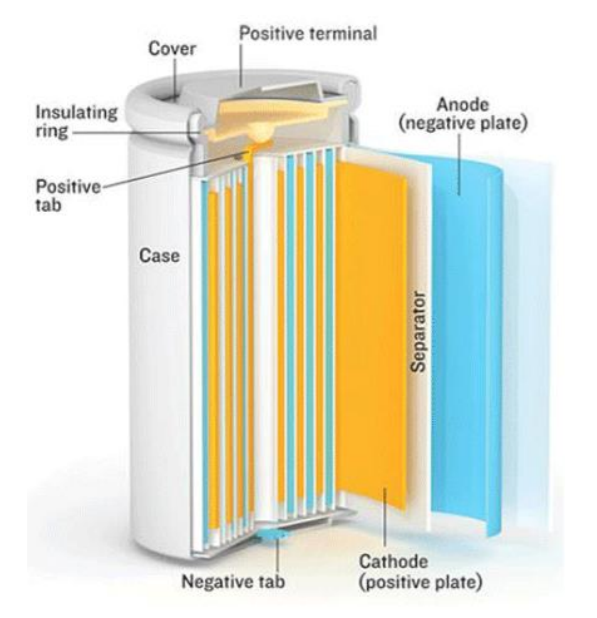
\includegraphics[width=0.5\linewidth]{Figures/cylindrical.PNG}
 	\caption{Schematic drawing of a cylindrical battery cell}
    \label{Fig:Cylindrical_Cell}
\end{figure}
It is said above, several safety options can be implemented in a cylindrical cell. The option to build internal safety mechanisms is quite an advantage over other types of cells since this can be fabricated during the battery creation. Most other cells can only have external safety devices to be attached to the external circuit, which requires assembly by users. Safety measures are explained in more detail in section \ref{Chap:Battery_Safety}. \\
Some disadvantages of cylindrical cells are that their size is limited, and thus their capacity. For large demanding applications, many of such batteries have to be combined. The assembly of such a battery pack may prove difficult and prone to errors. The optimal packing efficiency in a battery pack also is suboptimal. The packing efficiency can be approximated by the optimal packing of circles in a 2-dimensional field which is proven to be a hexagonal pattern \cite{optimal_packing} as seen in figure \ref{Fig:optimal_packing}.
\begin{figure} [H]
 	\centering	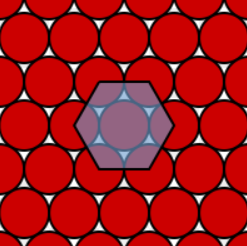
\includegraphics[width=0.5\linewidth]{Figures/optimal_packing.PNG}
 	\caption{Optimal packing of circles in a 2-dimensional space}
    \label{Fig:optimal_packing}
\end{figure}
The optimal packing is then calculated by formula \ref{Eq:optimal_packing}.
\begin{equation}
\frac{\pi}{\sqrt{12}} = 0.9069
\label{Eq:optimal_packing}
\end{equation}
Cylindrical cell packing ensures available cooling surface, though also a decrease of energy density in a battery pack. However, this energy density is further decreased since space is also lost by the metal enclosure and the empty center in a cylindrical cell. Additionally, the weight in a cylindrical cell battery pack is relatively high because of all the metal enclosures.\\
Even though cylindrical cells may thus seem undesirable for large battery packs, their cost, reliability and thermal management combined make for a combination that electric vehicle manufacturers choose for, like the Tesla company does for its vehicles \cite{battery_choice}.
\item Prismatic\\
The prismatic cell is basically a cylindrical cell but wound flattened. This makes for a more square shape which enables for a square metal housing. The square housing makes for a better packing density. They are however harder and more expensive to make than cylindrical cells and furthermore do not provide the same ability of incorporating certain safety mechanisms because of their square and asymmetric shape. Since the rise of pouch cells, Prismatic cells are becoming less popular now that the benefit of having a square shape is not unique to the prismatic cell anymore.
\item Pouch (LiPo)\\
Pouch cells have a distinctly different construction than cylindrical en prismatic cells have. Cylindrical and prismatic cells have a single sheet of battery layer that is wound up. Pouch cells on the other hand have a laminar layer. Battery layers are stacked upon each other and then sealed in an aluminum foil, with two metal connection terminal tabs sticking out. A schematic drawing is given in figure \ref{Fig:lipo_cell}, as well as an illustration of pouch cells.
\begin{figure}[H]
  \centering
  \subfloat[Pouch cell schematic.]{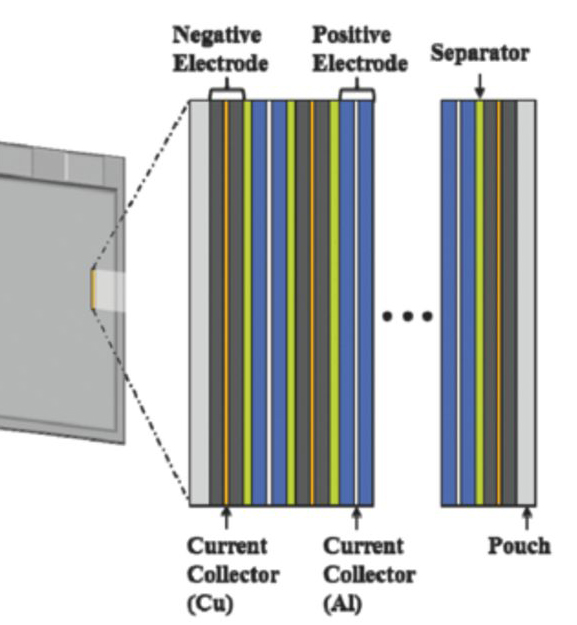
\includegraphics[width=0.5\textwidth]{Figures/Lipo_schematic.jpg}\label{Fig:lipo_schematic}}
  \hfill
  \subfloat[Pouch cells illustrated.]{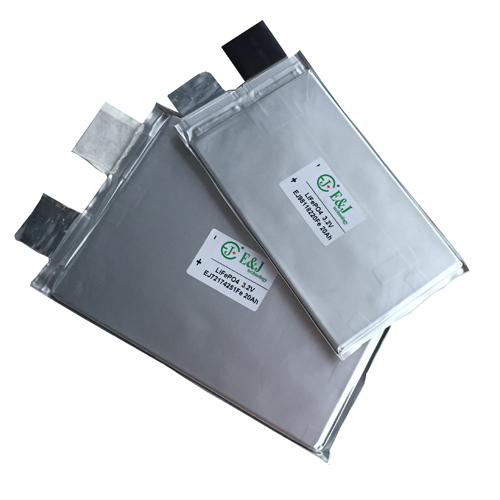
\includegraphics[width=0.5\textwidth]{Figures/Lipo_Cells.jpg}\label{Fig:lipo_cells}}
  \caption{Pouch cells}
  \label{Fig:lipo_cell}
\end{figure}
Because of their laminar origin, they can be created in many different shapes and sizes. Commercially they are almost always sold in rectangular shapes since this is cheap to produce and often a fit shape for their application. Their size is also variable from just as few as 10 mAh, up to more than 50Ah. This is because the layer sheets can be made as big as needed, and can also be stacked as many times as wished. This might cause thermal problems however, but it is possible if needed.\\
Pouch cells are optimized for power and energy density. Besides the active material, only current collectors and a thin aluminum foil is adding weight to the battery. This makes for a very weight and volume efficient design. A problem however is that a pouch cell has no hard metal casing, and thus is vulnerable to penetration. Also, lithium batteries swell as they age because of decomposition of active material. In hard metal casing this is suppressed, but in aluminum foil cased cells, batteries will expand. \\
Pouch cells have a very wide functionality. They are used in credit cards to provide power to its chip, but also function in electronic vehicles like the Nissan Leaf. \\
Commonly pouch cells are referred to as Lithium Polymer cells because of the laminar structure and their polymer separators. True Lithium Polymer cells however are cells with a polymer electrolyte. These however are not commercially available because of conductivity problems. The term LiPo for commercial cells as of now is thus incorrect \cite{Sequeira20103} \cite{lithium_batteries2}.
\item Solid-State\\
\textit{eerst meer informatie over zoeken, geen hoge prioriteit}
\end{enumerate}


%\begin{figure} [H]
% 	\centering
% 	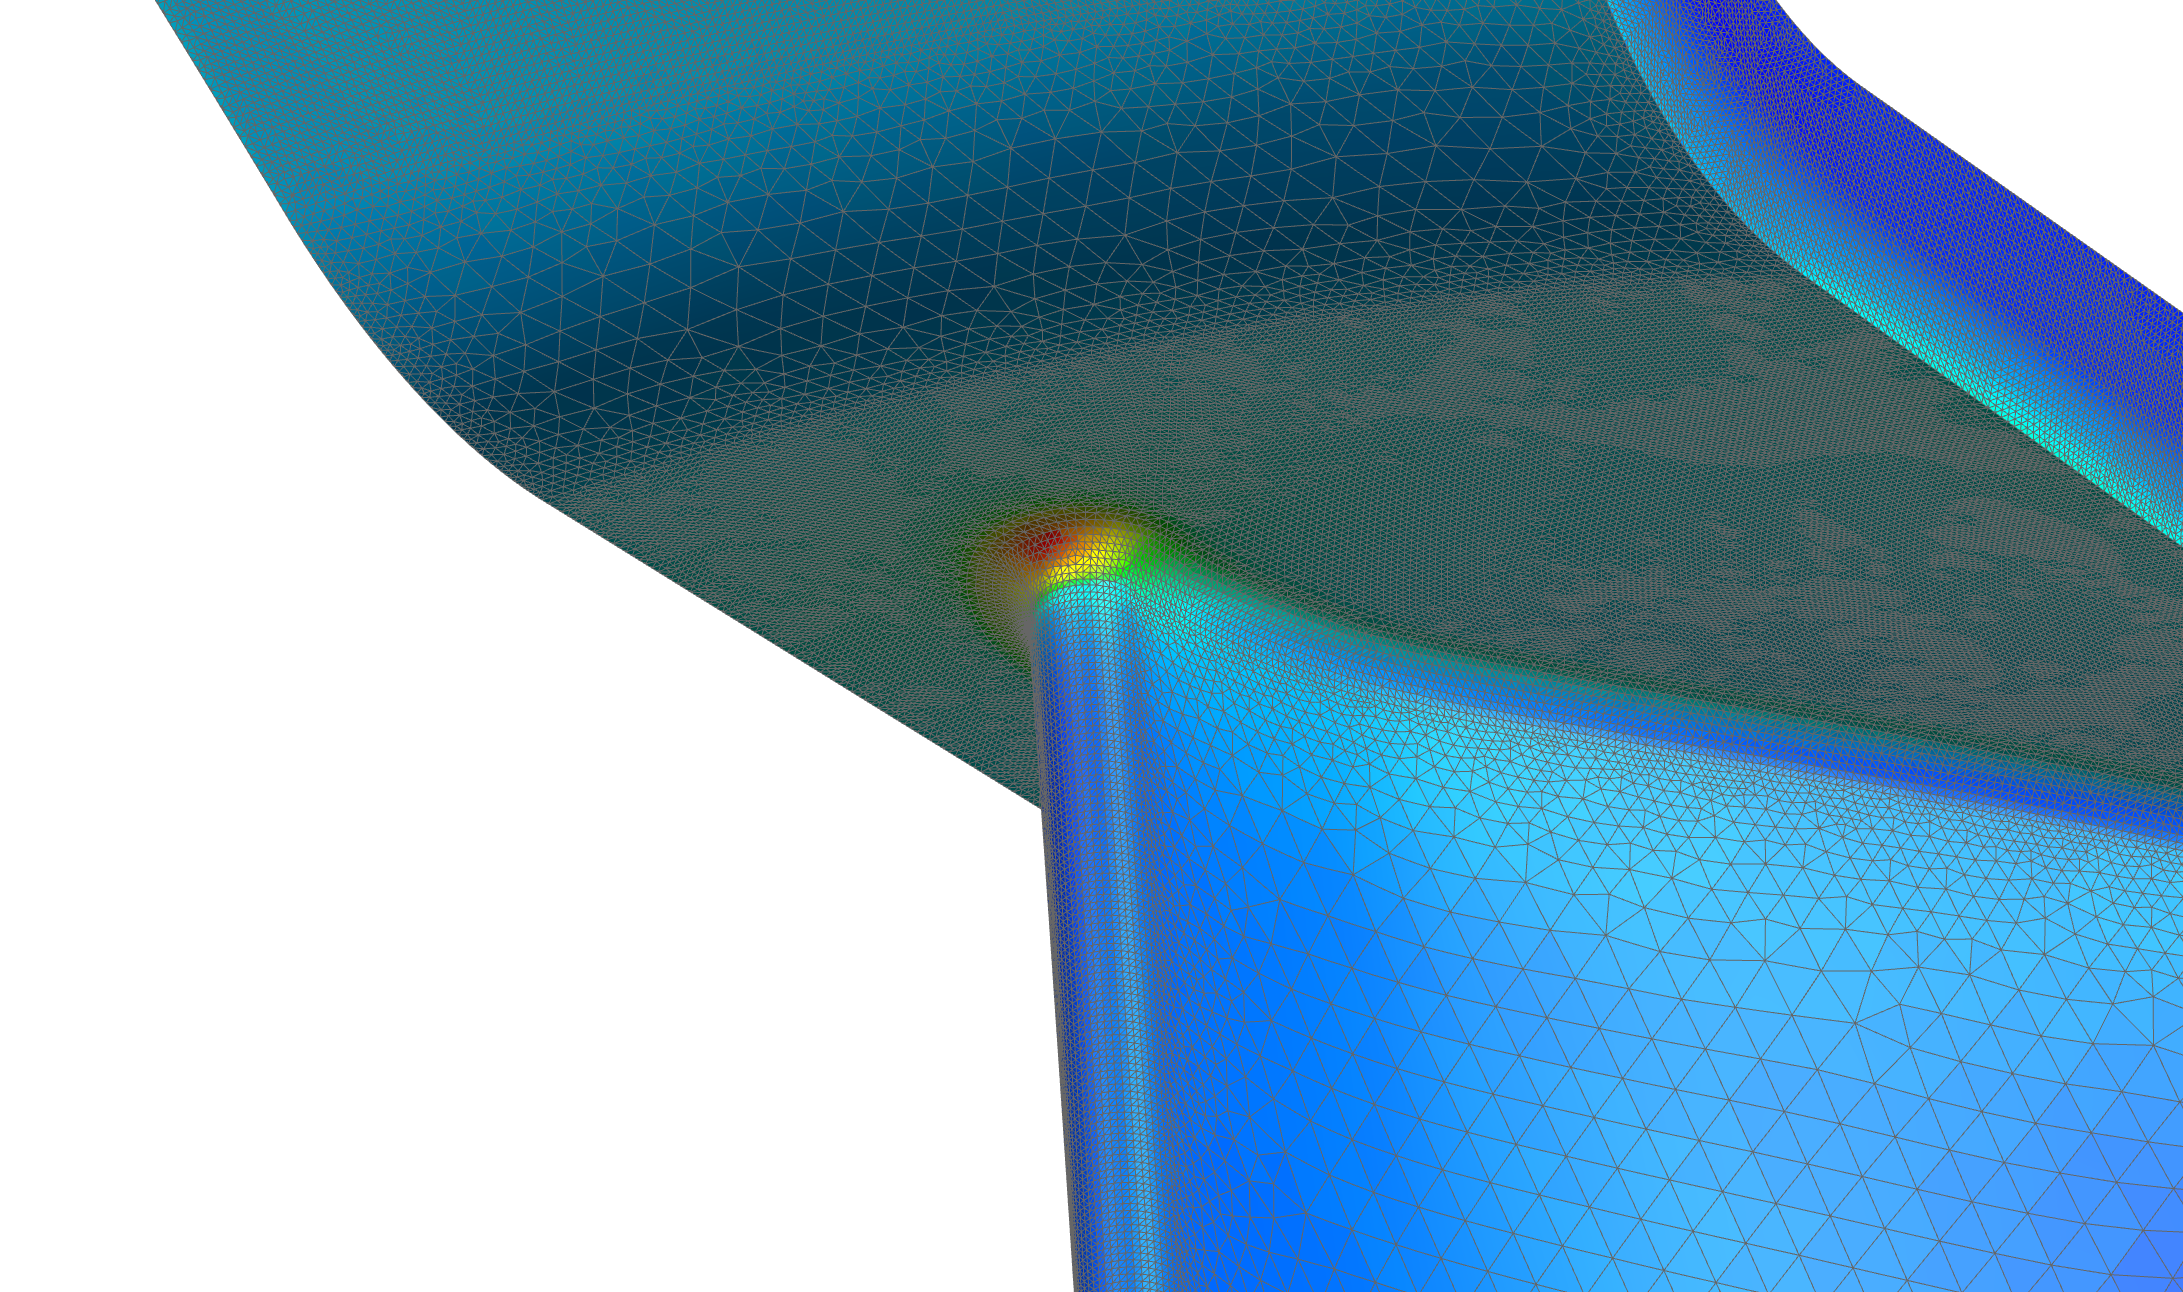
\includegraphics[width=0.8\linewidth]{Figures/stator_shutdown.png}
% 	\caption{Maximum stress during shut-down condition}
%    \label{stator1}
% \end{figure}

placeholder
\newpage